%%%%%%%%%%%%%%%%%%%%%%%%%%%%%%%%%%%%%%%%%%%%%%%%%%%%%%%%%%%%%%%%%%%%%%%%%%%%%%%%
%2345678901234567890123456789012345678901234567890123456789012345678901234567890
%        1         2         3         4         5         6         7         8

\documentclass[letterpaper, 10 pt, conference]{ieeeconf}  % Comment this line out
                                                          % if you need a4paper
%\documentclass[a4paper, 10pt, conference]{ieeeconf}      % Use this line for a4
                                                          % paper

\IEEEoverridecommandlockouts                              % This command is only
                                                          % needed if you want to
                                                          % use the \thanks command
\overrideIEEEmargins
% See the \addtolength command later in the file to balance the column lengths
% on the last page of the document



% The following packages can be found on http:\\www.ctan.org
\usepackage{graphics} % for pdf, bitmapped graphics files
\usepackage{epsfig} % for postscript graphics files
%\usepackage{mathptmx} % assumes new font selection scheme installed
%\usepackage{times} % assumes new font selection scheme installed
%\usepackage{amsmath} % assumes amsmath package installed
%\usepackage{amssymb}  % assumes amsmath package installed
\usepackage{listings}  % assumes amsmath package installed
\usepackage{caption}
\usepackage{subfigure}
\usepackage[utf8]{inputenc}

\title{\LARGE \bf
\hspace*{ 0.5 in}Comparing exact and heuristic methods for the  \newline Electronic Board Drilling-Traveling Salesperson problem
}

%\author{ \parbox{3 in}{\centering Huibert Kwakernaak*
%         \thanks{*Use the $\backslash$thanks command to put information here}\\
%         Faculty of Electrical Engineering, Mathematics and Computer Science\\
%         University of Twente\\
%         7500 AE Enschede, The Netherlands\\
%         {\tt\small h.kwakernaak@autsubmit.com}}
%         \hspace*{ 0.5 in}
%         \parbox{3 in}{ \centering Pradeep Misra**
%         \thanks{**The footnote marks may be inserted manually}\\
%        Department of Electrical Engineering \\
%         Wright State University\\
%         Dayton, OH 45435, USA\\
%         {\tt\small pmisra@cs.wright.edu}}
%}

\author{Giovanni Mazzocchin
\thanks{*This project has been done for a course on Combinatorial Optimisation held in Padua by professors Luigi De Giovanni and Marco Di Summa}% <-this % stops a space
}
%\thanks{*This work was not supported by any organization}% <-this % stops a space
%\thanks{$^{1}$H. Kwakernaak is with Faculty of Electrical Engineering, Mathematics and Computer Science,
% University of Twente, 7500 AE Enschede, The Netherlands
%        {\tt\small h.kwakernaak at papercept.net}}%
%\thanks{$^{2}$P. Misra is with the Department of Electrical Engineering, Wright State University,
%        Dayton, OH 45435, USA
%        {\tt\small p.misra at ieee.org}}%
%}


\begin{document}



\maketitle
\thispagestyle{empty}
\pagestyle{empty}


%%%%%%%%%%%%%%%%%%%%%%%%%%%%%%%%%%%%%%%%%%%%%%%%%%%%%%%%%%%%%%%%%%%%%%%%%%%%%%%%
\begin{abstract}
This report outlines some aspects of our work on the implementation of well-known exact and heuristic methods for the classic \textit{Electronic Board Drilling-Travelling Salesperson} problem.
Implementation issues and evaluation outcomes will be included as well.
\end{abstract}


%%%%%%%%%%%%%%%%%%%%%%%%%%%%%%%%%%%%%%%%%%%%%%%%%%%%%%%%%%%%%%%%%%%%%%%%%%%%%%%%
\section{INTRODUCTION}
\subsection{The problem}
This assignment comes from a real-world scenario: \newline \textit{a company produces boards with holes used to build electric frames. Boards are positioned over a machine and a drill moves over them, stopping at some desired positions
and drilling holes. Given the holes' positions on the board, we are supposed to determine the sequence of holes that minimises the total drilling time, taking into account
that the time required for making a hole is constant.} \newline 
This description's similarity to the more famous \textit{Traveling Salesperson problem} is noteworthy: actually,
they can be thought of as the same problem.
\subsection{The project} 
As the title suggests, our work is made up of two main parts:
\begin{itemize}
\item the first part comprises a tiny C++ program that utilises \textit{CPLEX}, a popular optimisation software which offers a library for this very language;
\item the second part is made up of a quite larger program implementing a \textit{Genetic Algorithm}. 
\end{itemize}

\section{Using \textit{CPLEX} to obtain an optimal solution}

\subsection{Data extraction}
The simplest yet essential component of this program is a class containing some methods able to read data from plain text files. These files should be generated according to the following template:
\begin{itemize}
\item the very first line should contain just a number standing for the problem's size;
\item the remainder of the file should contain a symmetric matrix of real numbers equipped with this meaning: the number in position \textit{(i,j)} represents the cost needed to move from hole (or \textit{city}) \textit{i} to city \textit{j}.
\end{itemize}

\subsection{Core components and remarkable issues}
The \textit{main} function works essentially as a starting point, namely, it does not perform anything remarkable except for calling our \textit{setupProblem} function (in \texttt{TSPSolver.h-cpp}) and carrying out some sanity checks.
\lstset{language=C++,
  basicstyle=\ttfamily,
}
\begin{lstlisting}[caption={Visit constraint}]
for (int i = 0; i < data.n; i++){
 coefs[i] = 1.0;
 for (int j = 0; j < data.n; j++){
   idx[j] = i*data.n + j;
 }
 CHECKED_CPX_CALL(CPXaddrows,
    env, lp, 
    0, 1, data.n, &rhs, &sense[0], 
    &matbeg[0], &idx[0], &coefs[0],
    NULL, NULL);
}
\end{lstlisting} 
With respect to variables and corresponding coefficients, we resorted to plain STL 
\textit{vectors}. As regards variables' ordering, we arbitrarily put the \textit{y}'s before the \textit{x}'s; note that we must take this priority into account for the sake of a correct access to variables and coefficients. Listing 2
shows a sort of "preamble" which is quite common before any constraint.
\begin{lstlisting}[caption={Important data structure declarations}]
const int x_init_index = data.n*data.n;
std::vector<int> idx(data.n);
std::vector<double> coefs(data.n);
\end{lstlisting}
In the above code extract, \texttt{x\_init\_index} represents the index where
the \textit{x} variables start from: it is equal to the square of the problem's size due to the fact that every \textit{y} has two indices. The second line declares a vector, \texttt{idx} (whose size corresponds to the problem's dimension), which will store all the variables the following constraint will make use of. On the other hand, \texttt{coefs} will store the coefficients related to the variables in question.

\subsection{Outcomes: reached optima and execution times}
In order to evaluate this first part, we used some reference random instances (which will be used by the second part as well) our program can be run against. \newline Table 1  gives insight into this program's efficiency and effectiveness.
\begin{table}[h]
\caption{Results for the first part}
\label{table_example}
\begin{center}
\begin{tabular}{|c|c|c|}
\hline
\textbf{Size of the problem} & \textbf{Optimum} & \textbf{Time (in seconds)} \\
\hline
12 &  66.4 &  0.38\\
\hline
26 & 937 & 0.85 \\
\hline
42 & 699 & 14.5\\
\hline
48 & 10628 & 24.5 \\
\hline
60 & 629.8 & 78.7 \\
\hline
100(a) & 21282 & 370 \\
\hline
100(b) & 22141 & 970 \\
\hline
200 & unknown & too large\\
\hline
\end{tabular}
\end{center}
\end{table}

\section{Approximating the optimum through Genetic algorithms}
The exact approach we described so far turns out to be quite unwieldy for attacking large instances, due to Simplex' inherent high time complexity.  
This sad news has prompted researchers to develop some \textit{heuristics} 
which should be able to yield approximate yet good solutions. A general method among these heuristics is the one we encounter in \textit{Genetic algorithms}.

\subsection{Generic steps} 
A traditional Genetic Algorithm for optimisation problems can be summarised as follows:
\begin{enumerate}
\item devise a suitable \textbf{encoding} for solutions (a.k.a. \underline{individuals}, hereafter these words will be interchangeable);
\item generate an initial \textbf{population}, i.e., a set of solutions;
\item \texttt{Loop}:
\item \hspace*{ 0.2 mm} \underline{select} couples (or groups) of \textbf{parent} solutions;
\item \hspace*{ 0.2 mm} generate an \textbf{offspring} thanks to \underline{recombination};
\item \hspace*{ 0.2 mm} evaluate new solutions' \textbf{fitness} (this concept will be \hspace*{ 0.2 mm} clarified later on);
\item \hspace*{ 0.2 mm} \underline{replace} current population using the offspring;
\item \texttt{Until:} a sensible stopping criterion;
\item \texttt{return} the best solution altogether.
\end{enumerate}

\subsection{Solution encoding and Fitness function}
The chosen encoding was the so-called \textit{path-representation}, according to which solutions can be seen as sequences of visited holes. \newline
As for the \textit{fitness} function, we decided not to use anything beyond the given objective function's value. Furthermore, we should say that we did not come across any viable alternative.

\subsection{Generating an initial population}
The first issue we face is generating a population as a good starting point for our algorithm. In this work we chose two strategies: the first leaves everything to chance, creating a random pool of feasible solutions the algorithm can start from, whereas the latter performs some \textit{local search} (namely a certain amount of iterations with \textit{Simulated Annealing}) on few (10\%) individuals, so that hopefully (but we do know that Simulated Annealing accomplishes its goal) the "genetic loop" is provided with a higher-quality initial population. Sometimes the latter technique will be referred to as "smart initialisation".
\begin{lstlisting}[caption={Code within main annealing loop, from \texttt{TSPPopulation.cpp}}]
double neighbourVal=evaluate(neighbourSol);   
double probability;
double diff = neighbourVal-currentSolVal;
if (neighbourVal < currentSolVal){
 double exponentialVal=exp(-(diff)/temp); 
 double probability = 1;
 if (exponentialVal < 1){
   probability = exponentialVal;
 }
 probability = probability * 100;    
 int prob_indicator = distr(rg);		
 if (prob_indicator < probability){   					
   population[i] = neighbourSol;
 }				
}
// temperature's drop
if (k == temp_thresh_1){
 temp = temp / 2;
}
\end{lstlisting}

\subsection{Selecting individuals for mating}
First of all, we should choose whether we want to perform mating on pairs
or larger-sized groups of individuals. We decided to implement the former option due to its simplicity and overall effectiveness. \newline
Plenty of selection criteria have been proposed in the literature: our choice fell on \textit{Tournament Selection}, whose pseudocode is given below: \newline\newline
\texttt{\textit{First step}: choose k individuals from the population at random
\newline \textit{Second step}: choose the best individual from the 
tournament with probability p
\newline \textit{Third step}: choose the second best individual 
with probability $p*(1-p)$
\newline \textit{N-th step}: choose the n-th best individual 
with probability $p\times((1-p)^{(n-2)})$}
\newline\newline
It can be shown that this strategy does not suffer from any bias towards "super-individuals" (that is, individuals endowed with better fitness), since it is easy to realise its independence from individuals' fitness values.


\subsection{Recombining individuals through Crossover}
As far as descendants' generation is concerned, we know we can carry it out thanks to various kinds of \textit{Crossover operators}. Generally speaking, we
could think of Crossover as a way to include a combination of parents' features into a child. As we have seen in the context of selection, there are lots of proposed operators here as well, which may vary in cost and
effectiveness. The latter requirement matters particularly in the setting we are working on: in fact, any operator that generates an offspring without being concerned about its feasibility would not be deemed as much effective.
We wrote the code both for \textit{Partially-Mapped Crossover} (Goldberg and Lingle) and \textit{Order Crossover} (Oliver et al., Goldberg), but since the former operator does not enforce feasibility, we are more amenable to go through the latter's steps, which are listed below:
\begin{enumerate}
\item randomly select a substring from a parent;
\item produce a proto-child by copying the substring into the
its corresponding position;
\item discard (from the second parent) the holes which have already been put in the substring. The remaining sequence contains the holes eligible to enter the proto-child;
\item place the holes into the unfixed positions of the proto-child proceeding from left to right. The order of the holes stemming from the second parent must be preserved.
\end{enumerate}


\begin{lstlisting}[caption={Order Crossover, in \texttt{TSPCrossover.cpp}}]
for (int i = 1; i < sol_size - 1; i++){
 if (counter1==fst_cut_ind_rnd){
  counter1=counter1+zoneSize;
 }
 if (counter2==fst_cut_ind_rnd){
  counter2=counter2+zoneSize;
 }
 it_indicator=find(conflictZone.begin(),
  conflictZone.end(),parent1[i]);
 if(it_indicator==conflictZone.end()){
  child1.sequence[counter1]=parent1[i]; 		                          
 }
}		
\end{lstlisting}

\subsection{Generational replacement}
One of the components needed by evolution is \textit{Generational Replacement}. With lack of any sensible replacement, evolution would get stuck to inadequate individuals. \newline 
The kind of strategy we adopted is called \textit{Best Individuals Replacement}. The aspect that drove us toward this method was its clear general description, which can be summarised straightforwardly with this sentence: \newline
\textit{generate \textbf{R} new individuals from \textbf{N} old ones, then keep the best \textbf{N} among the total \textbf{N + R}}. \newline
We achieved this method's goal by means of plain vector concatenation and sorting. In particular, the concatenation consists in appending the current offspring to the current population (which are both represented with vectors). The resulting vector is then sorted using an appropriate comparator. Efficiency reasons forced us to dispose of the worst 3\% of the resulting vector; this trick let us save up to minutes of computation time. Thus, the outcomes we will talk about will always refer to runs that take advantage of the trick mentioned above.
\begin{lstlisting}[caption={Best individual replacement, in \texttt{TSPPopulation.cpp}}]
TSPSolution repPop(vector offspring){ 
 population.insert(population.end(), 
    offspring.begin(),offspring.end());
 TSPSolutionComparator tspSolComp;
 sort(population.begin(),population.end(),
    tspSolComp);
}		
\end{lstlisting}


\subsection{Exploiting mutation to avoid premature convergence}
It is well known that lack of \textit{mutation} occurrence would make our algorithm doomed to be characterized by poor diversification. As a matter of fact, \textit{diversification} becomes necessary in order to escape from premature convergence, that is to say, ending up with a population made up of excessively similar individuals (\textit{genetic drift}). \newline
Therefore we are forced to introduce mutations, which obviously should occur seldom enough. Thanks to much painstaking tuning and testing, we found out that a fixed 0.2\% mutation probability (then multiplied by three during the very last 5\% of total generations) drives to decent results. Thus, hereafter we will stick to this value. \newline
As in the case with other genetic steps, there are many ways to perform mutation on an individual. Trial and error led us to choose \textit{2-opt} moves (namely, reversal of random substrings); however, our first choice consisted in performing random swaps between couples of holes (with very poor results which will not be reported). \newline
At last, it is worthwhile to mention that mutations could occur both on the initial population ("initial" is referred to a specific generation) and on its offspring.
\begin{lstlisting}[caption={2-opt move, in \texttt{TSPCrossover.h}}]
void doMutation(TSPSolution& individual){
 TSPSolution tmpSol(individual);
 for(int i=fstIndex;i<=sndIndex;i++){
   individual.sequence[i]=tmpSol[...];
 }
}
\end{lstlisting}

\section{Outcome analysis}
In this section we will focus on outcomes and data representation. In the last section of the paper, called \textit{Plots}, we will show two graphs per instance, whose aim is to show how quality and running time vary depending on the number of generations, given a fixed chosen number of individuals. Medium-sized instances have been attacked using both pure randomness and some local search in initialisation. On the other hand, bigger instances have been attacked only by means of smart initialisation. \newline 
We remark on the fact that all the plotted data come from \textit{averages}, that is, the program has been run several times
after fixing some parameters and then an average of the results has been calculated. Further details about testing can be found in the appendix titled \textit{Practical Notes}. \newline
The analysed instances are exactly the same as the ones that
have been discussed in the first part of the paper. \newline
From now on, we proceed with a thorough analysis of the graphs.
\subsubsection{Small instances} fig. a), b), c), and d) show
the average outcomes for two specific $12\times12$ and $26\times26$ instances. Figures show evident quality improvements as long as the number of generations increases, with some exceptions that are due to (we believe) the stochastic nature of genetic algorithms. Up to now, running time is not an issue.
\subsubsection{Medium-sized instances} figures e) and f) come from a more complex background: this $42\times42$ instance has been tested both with and without Simulated Annealing. Thus, two lines have been plotted. Using Simulated Annealing (1000 iterations) to initialise even a small fraction of the starting population gave us remarkable improvements, notwithstanding a reduced population size. In fact, the 800-individual population was tested without Simulated Annealing, whereas the 500-individual one did take advantage of it.
\subsubsection{Large instances} figures g) and h) refer to the instance that had been named \textit{100a} in the first part.
Here we plotted only the results coming from a Simulated Annealing initialisation (6000 iterations), because its absence 
provided us with very poor results. These plots show that quality 
and running time start to become an issue.
\newline
A table with quality variances for some instances is given below:
\begin{table}[h]
\caption{Quality variance on different instances}
\label{table_example}
\begin{center}
\begin{tabular}{|c|c|c|c|c|}
\hline
\textbf{Size} & \textbf{Smart init. iter.} & \textbf{Population-Gener.} & \textbf{Variance}\\
\hline
42 &  0 & 800-400 & 1.37\%\\
\hline
42 & 1000 & 500-300 & 0.63\% \\
\hline
60 & 0 & 1500-500 & 1.77\%\\
\hline
60 & 4000 & 600-400 &  0.17\% \\
\hline
100b & 6000 & 1000-500 & 1.07\% \\
\hline
\end{tabular}
\end{center}
\end{table}

\section{CONCLUSIONS}
This practical work on combinatorial problems allowed us to grasp many fundamental concepts. First of all, we realised that exact methods do not always manage to give good solutions in an acceptable amount of time. Seeing the striking surge in running time beyond instances with 60 holes has been interesting as well. \newline 
As far as genetic algorithms are concerned, the results for smaller instances have been excellent both in term of quality and computation time. On the other hand, bigger instances required much more time to approach the optimum. Initialising some individuals by way of Simulated Annealing gave us a dramatic improvement for these instances. \newline However, we should always be aware of the fact that these heuristics give no optimality guarantee.


\addtolength{\textheight}{-12cm}   % This command serves to balance the column lengths
                                  % on the last page of the document manually. It shortens
                                  % the textheight of the last page by a suitable amount.
                                  % This command does not take effect until the next page
                                  % so it should come on the page before the last. Make
                                  % sure that you do not shorten the textheight too much.

%%%%%%%%%%%%%%%%%%%%%%%%%%%%%%%%%%%%%%%%%%%%%%%%%%%%%%%%%%%%%%%%%%%%%%%%%%%%%%%%



%%%%%%%%%%%%%%%%%%%%%%%%%%%%%%%%%%%%%%%%%%%%%%%%%%%%%%%%%%%%%%%%%%%%%%%%%%%%%%%%



%%%%%%%%%%%%%%%%%%%%%%%%%%%%%%%%%%%%%%%%%%%%%%%%%%%%%%%%%%%%%%%%%%%%%%%%%%%%%%%%
\section*{Practical notes}
Here the reader can find some important information regarding 
compilation and execution of the software.

%\subsubsection{First part}
\begin{itemize}
\item \textit{First part} 
%\renewcommand{\labelitemi}{$\star$}
\begin{itemize} 
\item \textbf{Compilation and execution}: run \texttt{make} in the folder called \textit{part1}, then launch \textit{./main instance\_file\_name}
from the same place. Instances can be found under \textit{part2/instance\_generator}.
\end{itemize}

%\subsubsection{Second part}
\item \textit{Second part}
%\renewcommand{\labelitemi}{$\star$}
\begin{itemize} 
\item \textbf{Compilation and execution}: compilation should be as easy as running \textit{make} in the folder called \textit{part2}.\newline 
In order to get some hints on how to run the program, launch \textit{./main} from the same directory; anyway, we have provided you with some handy scripts which will be discussed below.
\item \textbf{Instances}: the directory named \textit{instance\_generator} contains some instances we found in \textit{TSPLIB}, a library of sample instances for well-known combinatorial problems.
\item \textbf{Testing}: some \textit{shell scripts} are present under the directory named \texttt{results}. There exists a script named \textit{launchX.sh} (where \textit{X} is the instance's size) for each instance. In order to run them, you are obliged to give them execution permissions running the following command: \textit{chmod +x script\_name}. \newline
These scripts accept two parameters from the command line: first, they require the problem's known optimum, then the name of an output file which will store their output. \newline We decided to leave some parameters such as \textit{population's size} and \textit{number of generations} hard-coded. \newline
After receiving all the data, these scripts run our program  several times (up to 49 for smaller instances, whereas we stopped to 30 for the bigger ones), so that we can calculate statistical parameters (such as mean and variance) afterwards.
This large amount of testing is required since the algorithms' behaviour is stochastic in nature.
\end{itemize}
\end{itemize}

\section*{Plots}
Some plots (along with understandable captions) are provided in the next pages.
\clearpage

\begin{figure}[ht!]
     \begin{center}
%
        \subfigure[Quality for a $12\times12$ instance]{%
            \label{fig:first}
            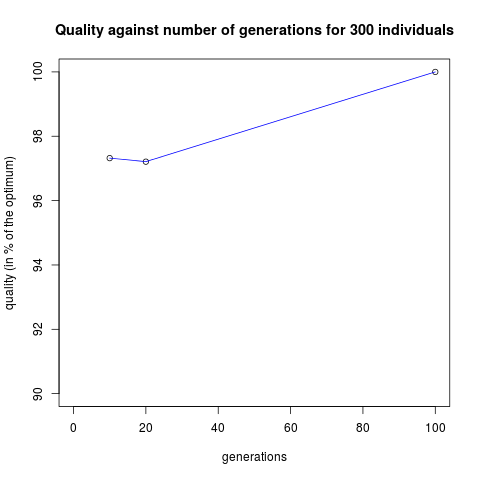
\includegraphics[width=0.5\textwidth]{quality12}
        }%
        \subfigure[Running time for a $12\times12$ instance]{%
           \label{fig:second}
           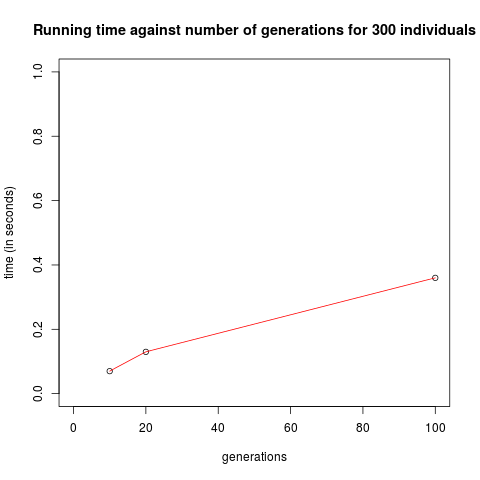
\includegraphics[width=0.5\textwidth]{time12}
        }\\ %  ------- End of the first row ----------------------%
        \subfigure[Quality for a $26\times26$ instance]{%
            \label{fig:third}
            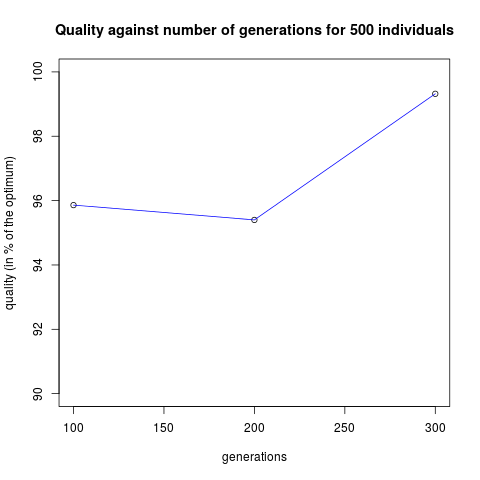
\includegraphics[width=0.5\textwidth]{quality26}
        }%
        \subfigure[Running time for a $26\times26$ instance]{%
            \label{fig:fourth}
            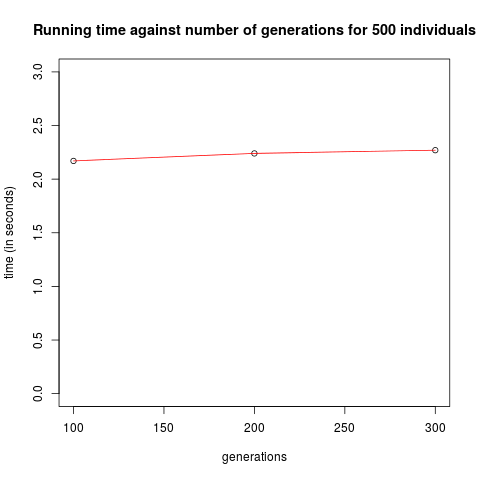
\includegraphics[width=0.5\textwidth]{time26}
        }%
%
    \end{center}
    %\caption{%
     %   }%
   \label{fig:subfigures}
\end{figure}

\clearpage 
\begin{figure}[ht!]
     \begin{center}
%
        \subfigure[Quality for a $42\times42$ instance]{%
            \label{fig:first}
            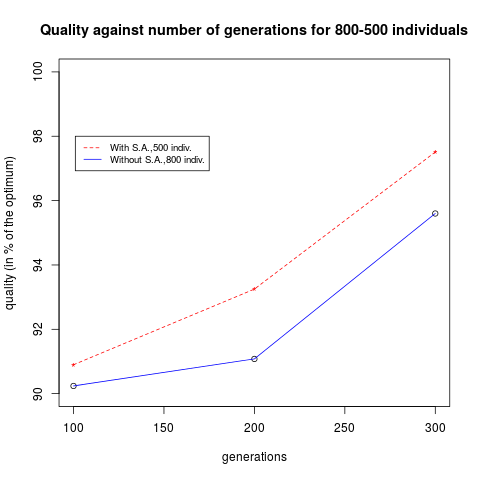
\includegraphics[width=0.5\textwidth]{quality42}
        }%
        \subfigure[Running time for a $42\times42$ instance]{%
           \label{fig:second}
           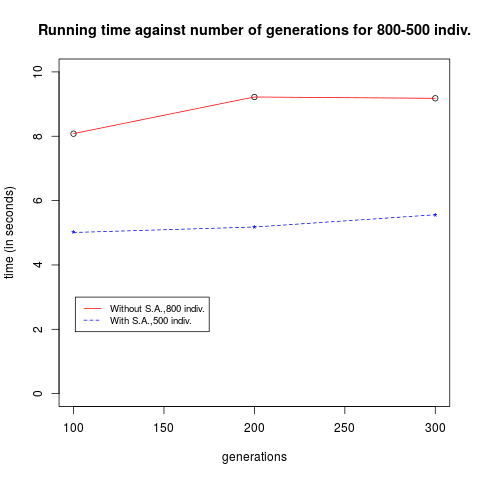
\includegraphics[width=0.5\textwidth]{time42}
        }\\ %  ------- End of the first row ----------------------%
        \subfigure[Quality for a $100\times100$ instance]{%
            \label{fig:third}
            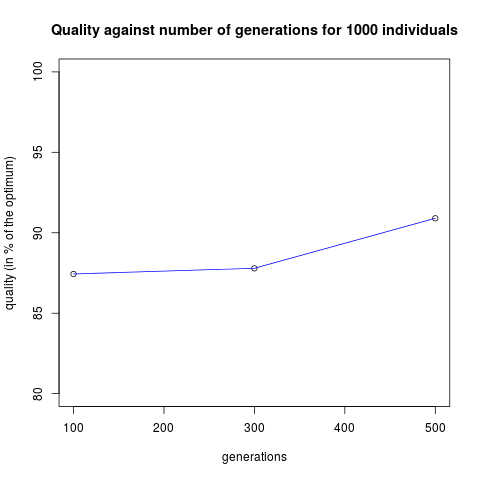
\includegraphics[width=0.5\textwidth]{quality100a}
        }%
        \subfigure[Running time for a $100\times100$ instance]{%
            \label{fig:fourth}
            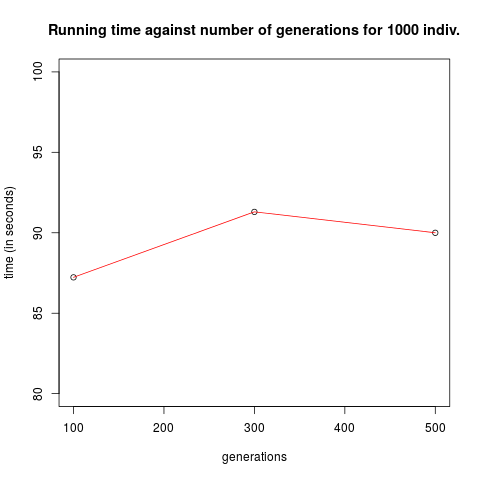
\includegraphics[width=0.5\textwidth]{time100a}
        }%
%
    \end{center}
    %\caption{%
     %   }%
   \label{fig:subfigures}
\end{figure}



%%%%%%%%%%%%%%%%%%%%%%%%%%%%%%%%%%%%%%%%%%%%%%%%%%%%%%%%%%%%%%%%%%%%%%%%%%%%%%%%
\clearpage 
\begin{thebibliography}{99}
\bibitem{c1} Jean-Yves Potvin, Genetic algorithms for the
Traveling Salesman Problem,
Centre de Recherche sur les Transports, Université de Montréal,
C.P. 6128, Succ. Centre-Ville, Montréal, Québec, Canada H3C 3J7 
\end{thebibliography}

\end{document}
